\documentclass[12pt]{article}
\title{Results Analysis}
\author{Mostafa Rizk}

\usepackage{graphicx}
\usepackage{subfig}
\usepackage[margin=1.5in]{geometry}
\usepackage{fancyhdr}
\usepackage{url}

\fancyhead{}
\fancyfoot{}
\fancyfoot[R]{\thepage}

\pagestyle{fancy}
\begin{document}
\maketitle
\tableofcontents

\section{Executive Summary}

\section{Analysis}
		
We have faced difficulty evolving cooperation in the SlopeForaging multi-agent setting. We conducted an analysis using Oller et al's rwg benchmarking approach \cite{oller:2020:arXiv} to understand the nature of the difficulties posed by this environment. We hope this will provide insight into what changes need to be made to our approach in order to produce the desired behaviour. All experiments used a homogeneous team, rewarded at the team level. Heterogeneous teams and individual rewards are not considered yet.\\

In each experiment, we sampled 50,000 genomes from a normal distribution with a mean of 0 and unit variance. Each genome was evaluated for 5 episodes. In any instance where hidden layers were used, we used 4 hidden units. We plot a) all the trials in sorted order, b) the variance of all trials and c) the distribution on a log scale.
		
\subsection{FFNN vs RNN}

We started our experiments with the simplest possible architecture, a FFNN with no bias, no hidden layers and linear activation (i.e. the identity function). We added up to two hidden layers, then repeated with bias, making for a total of 6 experiments. We then repeated the 6 experiments with a RNN.\\

For the FFNN, the scores are overwhelmingly poor, all falling into the leftmost bucket of the distribution plot as we see in Figure \ref{fig:ffnn_linear}. We see that the mean curve is very flat, with very little variance. The results appear to be almost identical regardless of the number of hidden layers. We discovered later, according to Theorem 1.5.1 in \cite{aggarwal:2018:springer}, that hidden layers do not add computational power if the activation function is linear. We repeated these experiments in Section \ref{non-linear} with various non-linear activations. We also find that adding a bias neuron does not make a difference to the results.\\

Most significantly, we see that an RNN performs overwhelmingly better than a FFNN. This makes sense because the environment is partially observable; an agent can only see 1 tile in any direction. A recurrent architecture means an agent can act on sequences of observations rather than individual observations, giving it an advantage over an agent with no memory. Presumably, if the agent's sensing radius was expanded to include the entire arena then the FFNN would perform similarly to the RNN.\\ 

Most of the RNN solutions are still quite poor, with the majority again fitting in the leftmost bucket in the distribution histogram. The mean curve is, as with the FFNN, very flat as we see in Figure \ref{fig:rnn_linear} but there is a spike at the end, denoting a very small proportion of samples that perform much better than the others. We can also see that the variance is higher for higher means which indicates that genomes that score well do not do so consistently across all episodes.\\

On a more fundamental level, we learn that the environment, independent of architecture, is challenging in a way that is similar to the MountainCar \cite{MountainCar} environment investigated by Oller et al \cite{oller:2020:arXiv}. The plots are very similar with most solutions being equally poor and very few demonstrating a successful behaviour. This is likely because both environments have a sparse reward. In the case of MountainCar, an agent must reach the top of the mountain to receive a score better than -200 and there are no rewards for partially successful intermediate behaviours. An agent that never moves is equivalent to one that stops just short of the goal. In SlopeForaging, an agent that travels up the slope, picks up a resource, carries it to the bottom of the slope and drops it just short of the nest is equivalent to an agent that oscillates back and forth between two tiles. A non-negative score can only be achieved if a resource is fully retrieved and there are no rewards for partially successful intermediate behaviours, so the task can not be learned incrementally.\\

In fact, the SlopeForaging task is actually more difficult for the following reasons:

\begin{itemize}
\item \textit{The observation and action spaces are larger}- An observation consists of 41 binary inputs and there are 6 discrete actions. Even the simplest FFNN would have 41x6=246 weights compared to (2x4) + (4x4) + (4x3) = 36 for the most complex controller used by Oller et al to solve MountainCar. 

\item \textit{The environment is partially observable}- Partial observability means a more complex architecture (RNN) is required.

\item \textit{The best solution isn't found even after 50,000 samples}- In MountainCar \cite{MountainCar}, the theoretical best score is close to 0 and the solutions generated by Oller et al approach this value, whereas in SlopeForaging, a team of specialists hardcoded with a cooperative strategy scores 157,000 but the best mean score of the solutions found by rwg is 39,879 and the best episode score is 52,642 (for a recurrent network). This is very far from the best known solution. It is even far from the best known generalist strategy, which scores 112,000. And all this is with 5 times more sampled solutions than Oller et al. All this is to say, the task is difficult to solve and, according to Oller et al's recommendations, may require an algorithm with a strong exploratory component.

\end{itemize}

\textbf{Main takeaway: The SlopeForaging task has similar attributes to MountainCar but is more difficult due to observation size, action space, partial observability and the cooperative nature of the task. Memory appears to be required for good performance but bias doesn't make a difference. A non-linear activation may be necessary for better results.}

\begin{figure}[!tbp]
  \centering
  % FFNN no-bias 0HL
  \subfloat{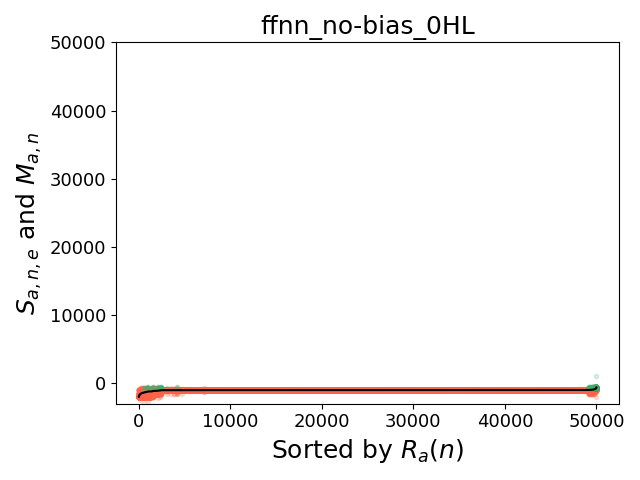
\includegraphics[width=0.3\textwidth]{ffnn_no-bias_0HL/ffnn_no-bias_0HL_score_trials_ordered_.png}}
  \hfill
  \subfloat{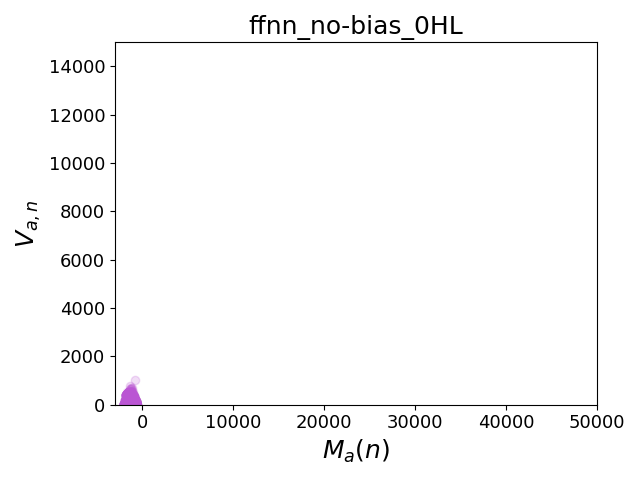
\includegraphics[width=0.3\textwidth]{ffnn_no-bias_0HL/ffnn_no-bias_0HL_variance_meanscore_.png}}
  \hfill
  \subfloat{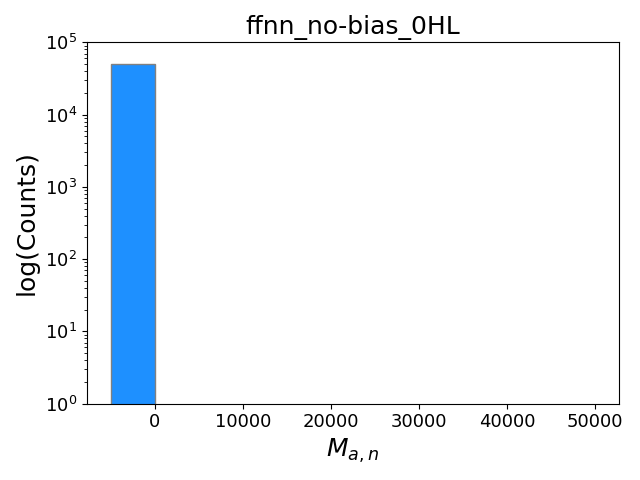
\includegraphics[width=0.3\textwidth]{ffnn_no-bias_0HL/ffnn_no-bias_0HL_all_scores_log_dist_.png}}
  
  % FFNN no-bias 1HL
  \subfloat{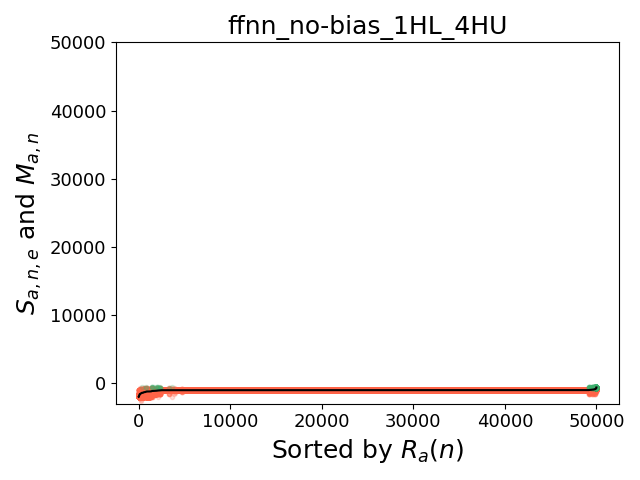
\includegraphics[width=0.3\textwidth]{ffnn_no-bias_1HL_4HU/ffnn_no-bias_1HL_4HU_score_trials_ordered_.png}}
  \hfill
  \subfloat{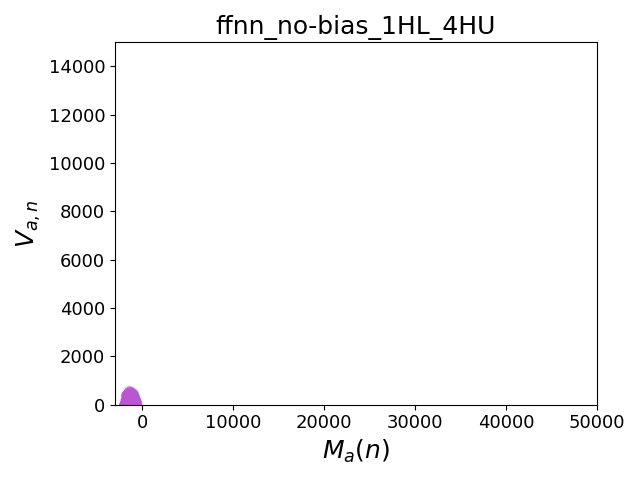
\includegraphics[width=0.3\textwidth]{ffnn_no-bias_1HL_4HU/ffnn_no-bias_1HL_4HU_variance_meanscore_.png}}
  \hfill
  \subfloat{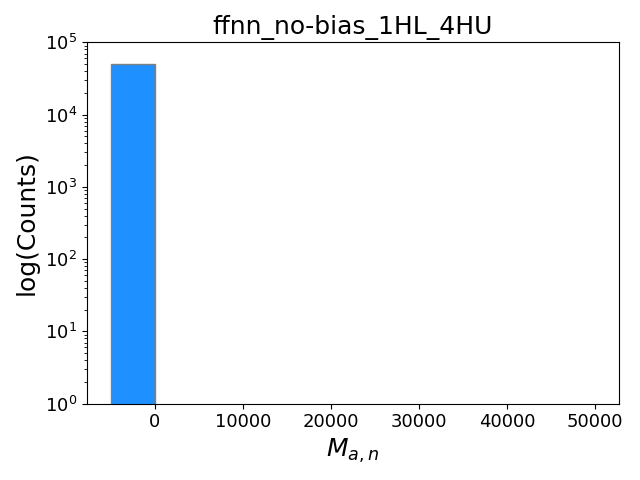
\includegraphics[width=0.3\textwidth]{ffnn_no-bias_1HL_4HU/ffnn_no-bias_1HL_4HU_all_scores_log_dist_.png}}

% FFNN no-bias 2HL
  \subfloat{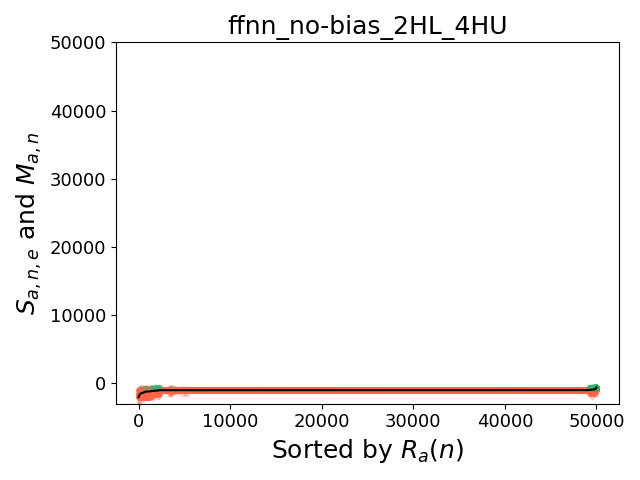
\includegraphics[width=0.3\textwidth]{ffnn_no-bias_2HL_4HU/ffnn_no-bias_2HL_4HU_score_trials_ordered_.png}}
  \hfill
  \subfloat{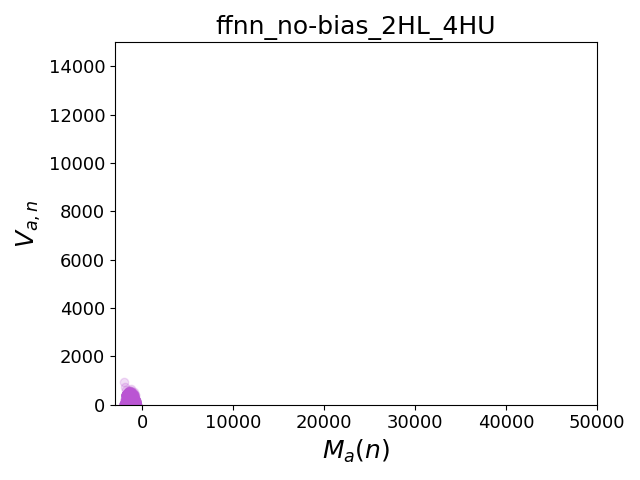
\includegraphics[width=0.3\textwidth]{ffnn_no-bias_2HL_4HU/ffnn_no-bias_2HL_4HU_variance_meanscore_.png}}
  \hfill
  \subfloat{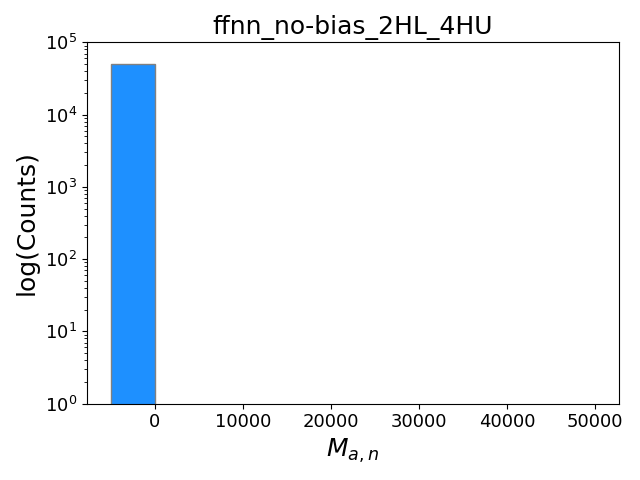
\includegraphics[width=0.3\textwidth]{ffnn_no-bias_2HL_4HU/ffnn_no-bias_2HL_4HU_all_scores_log_dist_.png}}
  
% FFNN bias 0HL
  \subfloat{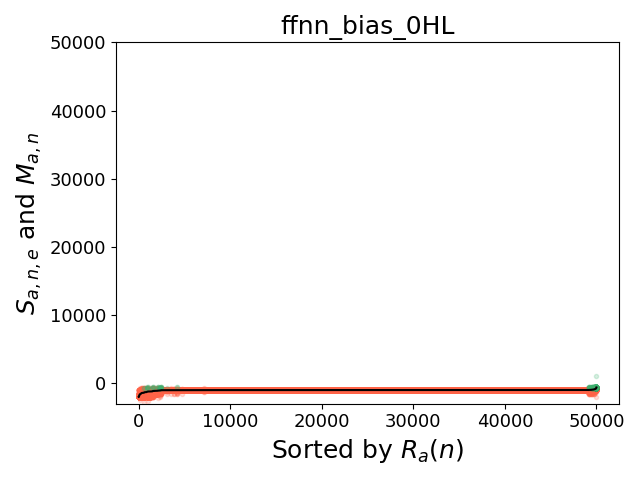
\includegraphics[width=0.3\textwidth]{ffnn_bias_0HL/ffnn_bias_0HL_score_trials_ordered_.png}}
  \hfill
  \subfloat{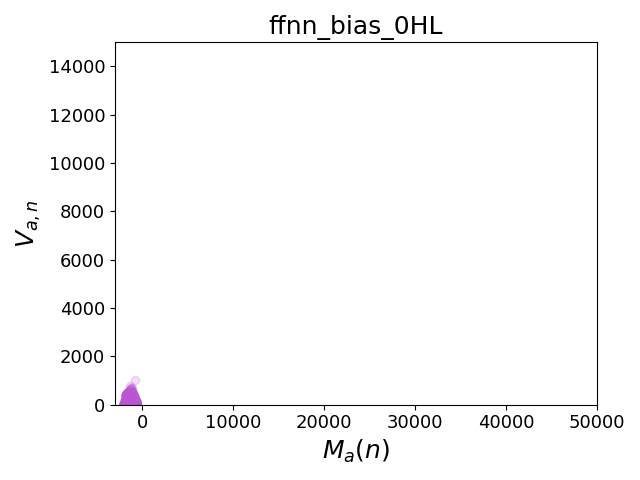
\includegraphics[width=0.3\textwidth]{ffnn_bias_0HL/ffnn_bias_0HL_variance_meanscore_.png}}
  \hfill
  \subfloat{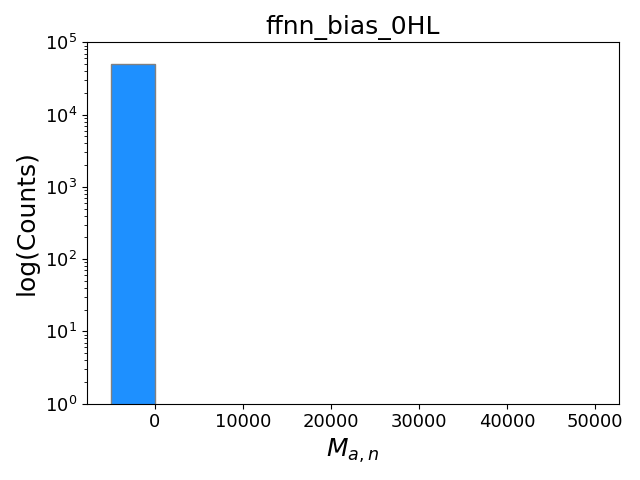
\includegraphics[width=0.3\textwidth]{ffnn_bias_0HL/ffnn_bias_0HL_all_scores_log_dist_.png}}
  
  % FFNN bias 1HL
  \subfloat{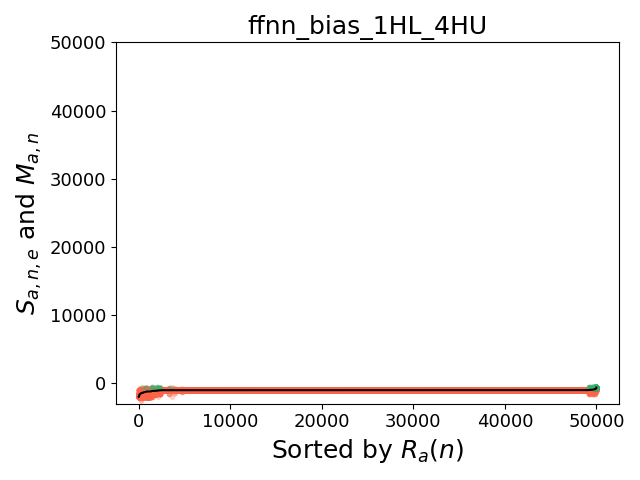
\includegraphics[width=0.3\textwidth]{ffnn_bias_1HL_4HU/ffnn_bias_1HL_4HU_score_trials_ordered_.png}}
  \hfill
  \subfloat{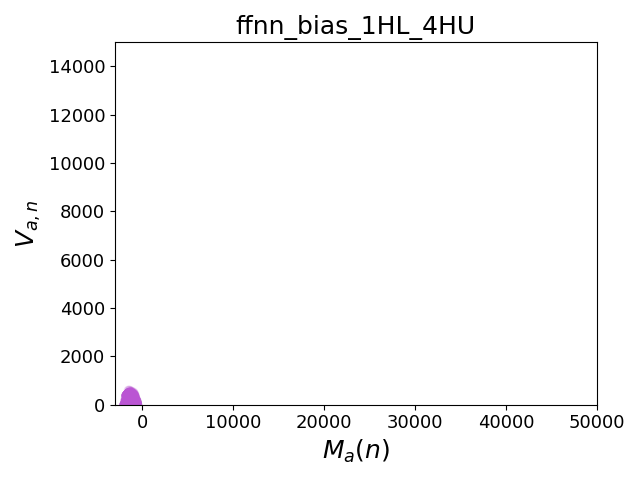
\includegraphics[width=0.3\textwidth]{ffnn_bias_1HL_4HU/ffnn_bias_1HL_4HU_variance_meanscore_.png}}
  \hfill
  \subfloat{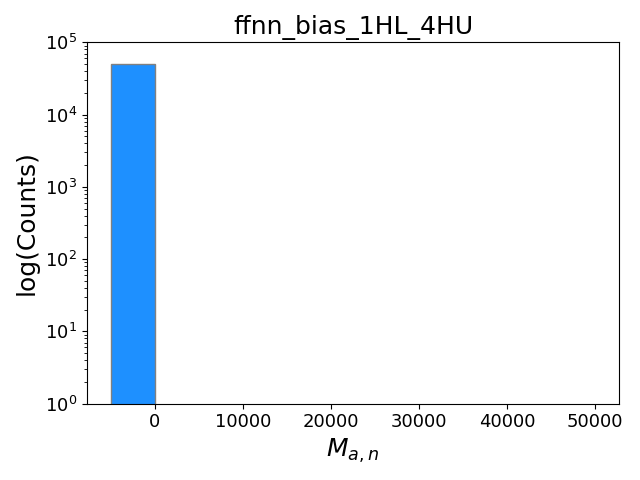
\includegraphics[width=0.3\textwidth]{ffnn_bias_1HL_4HU/ffnn_bias_1HL_4HU_all_scores_log_dist_.png}}

% FFNN bias 2HL
  \subfloat{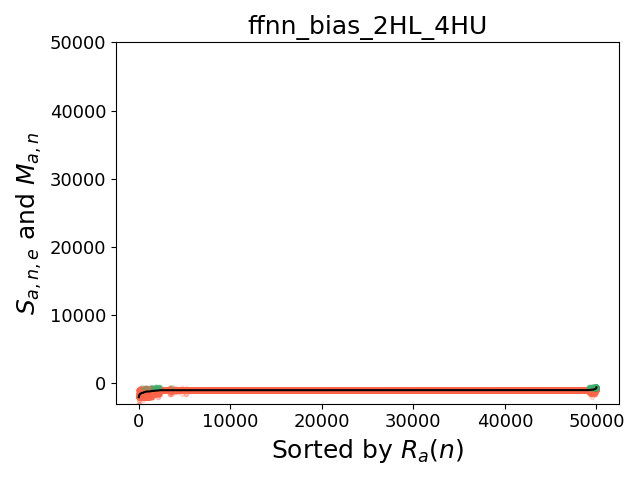
\includegraphics[width=0.3\textwidth]{ffnn_bias_2HL_4HU/ffnn_bias_2HL_4HU_score_trials_ordered_.png}}
  \hfill
  \subfloat{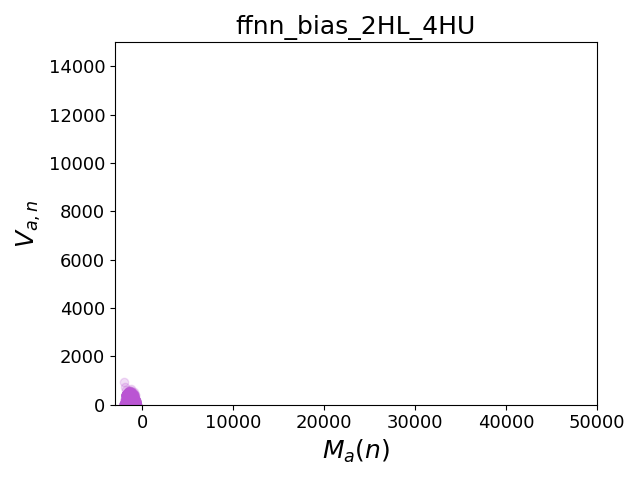
\includegraphics[width=0.3\textwidth]{ffnn_bias_2HL_4HU/ffnn_bias_2HL_4HU_variance_meanscore_.png}}
  \hfill
  \subfloat{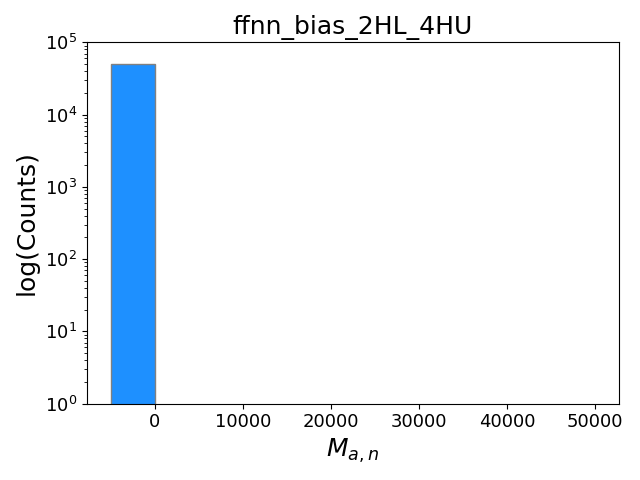
\includegraphics[width=0.3\textwidth]{ffnn_bias_2HL_4HU/ffnn_bias_2HL_4HU_all_scores_log_dist_.png}}  
  
  \caption{FFNN with linear activation}
  \label{fig:ffnn_linear}
\end{figure}

%%%

\begin{figure}[!tbp]
  \centering
  % RNN no-bias 0HL
  \subfloat{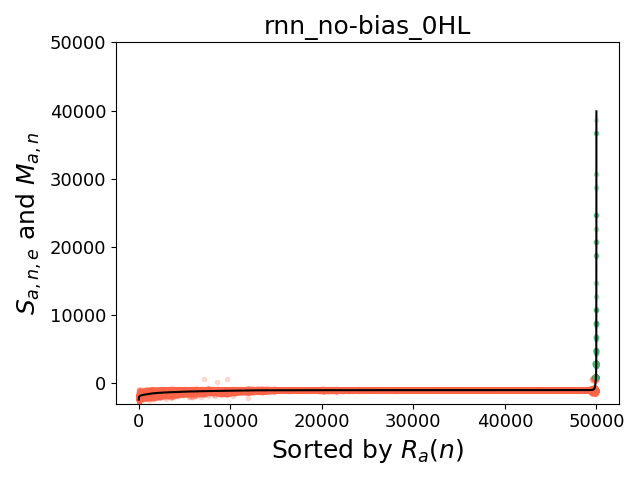
\includegraphics[width=0.3\textwidth]{rnn_no-bias_0HL/rnn_no-bias_0HL_score_trials_ordered_.png}}
  \hfill
  \subfloat{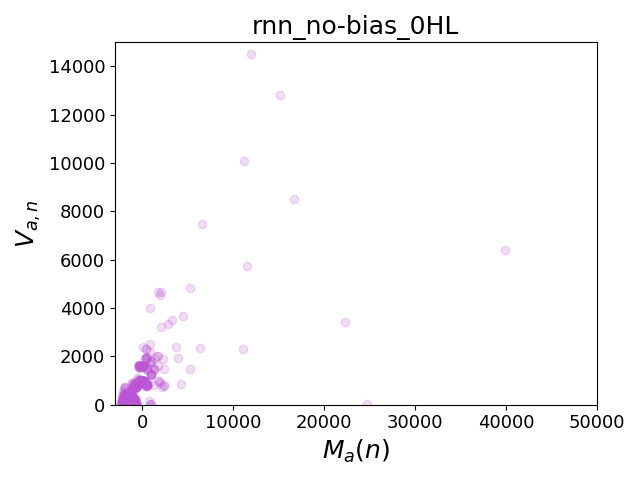
\includegraphics[width=0.3\textwidth]{rnn_no-bias_0HL/rnn_no-bias_0HL_variance_meanscore_.png}}
  \hfill
  \subfloat{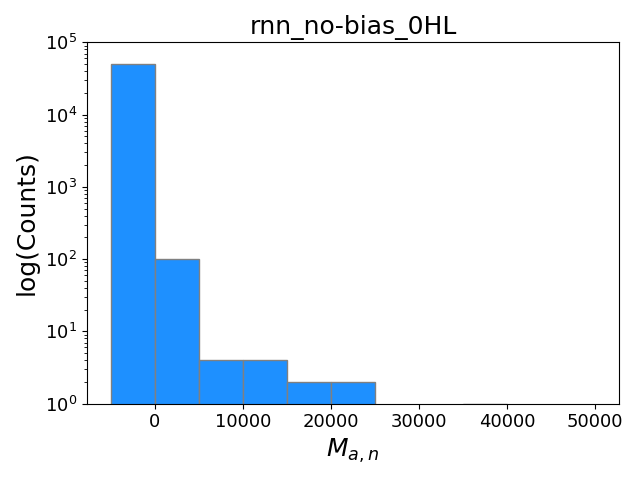
\includegraphics[width=0.3\textwidth]{rnn_no-bias_0HL/rnn_no-bias_0HL_all_scores_log_dist_.png}}
  
  % RNN no-bias 1HL
  \subfloat{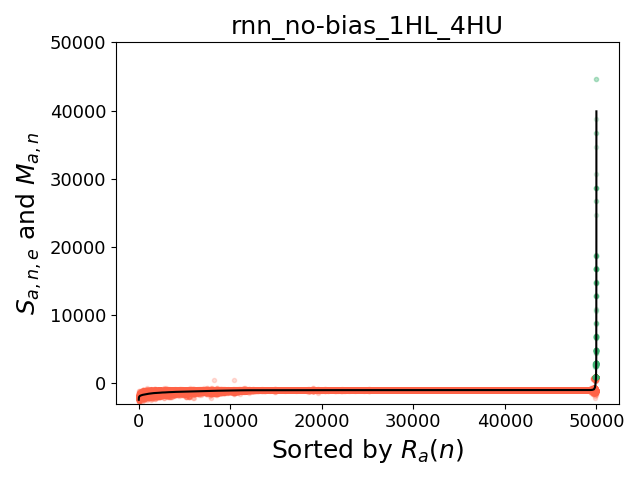
\includegraphics[width=0.3\textwidth]{rnn_no-bias_1HL_4HU/rnn_no-bias_1HL_4HU_score_trials_ordered_.png}}
  \hfill
  \subfloat{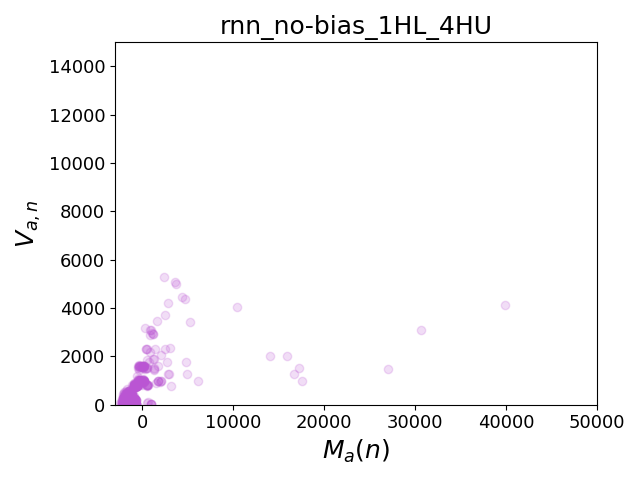
\includegraphics[width=0.3\textwidth]{rnn_no-bias_1HL_4HU/rnn_no-bias_1HL_4HU_variance_meanscore_.png}}
  \hfill
  \subfloat{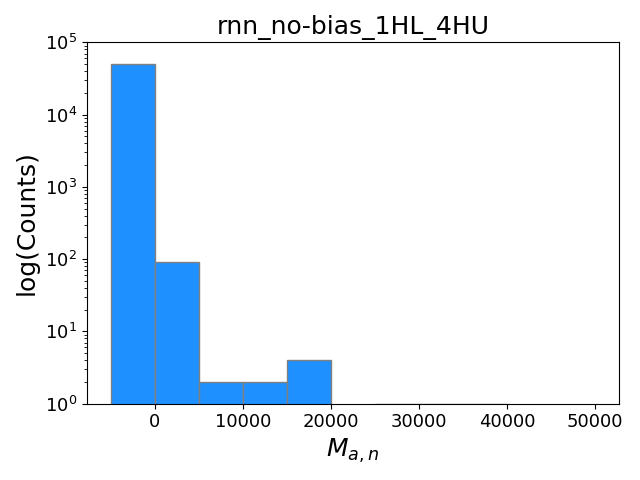
\includegraphics[width=0.3\textwidth]{rnn_no-bias_1HL_4HU/rnn_no-bias_1HL_4HU_all_scores_log_dist_.png}}

% RNN no-bias 2HL
  \subfloat{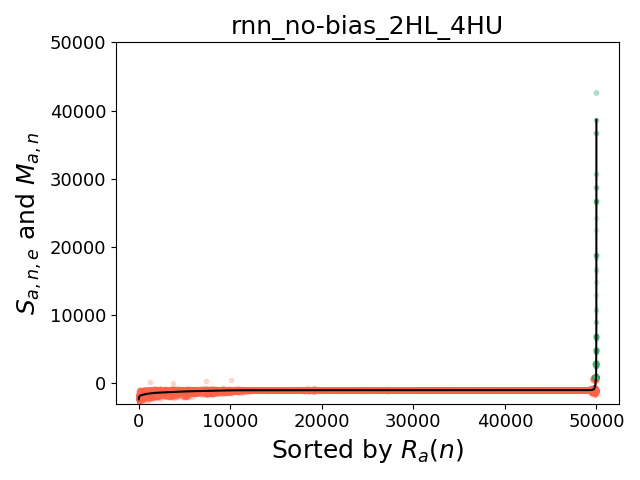
\includegraphics[width=0.3\textwidth]{rnn_no-bias_2HL_4HU/rnn_no-bias_2HL_4HU_score_trials_ordered_.png}}
  \hfill
  \subfloat{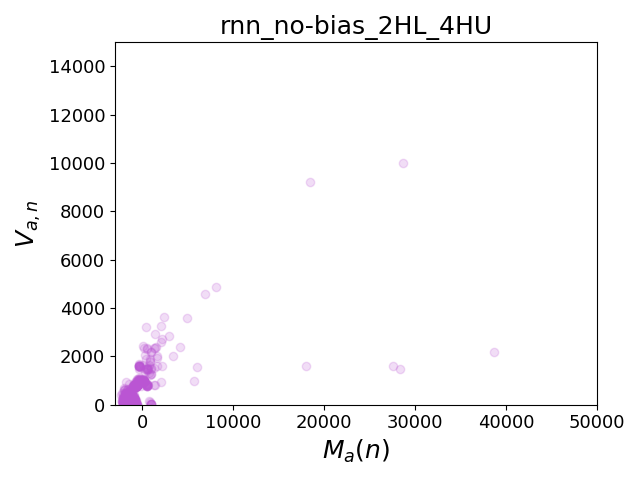
\includegraphics[width=0.3\textwidth]{rnn_no-bias_2HL_4HU/rnn_no-bias_2HL_4HU_variance_meanscore_.png}}
  \hfill
  \subfloat{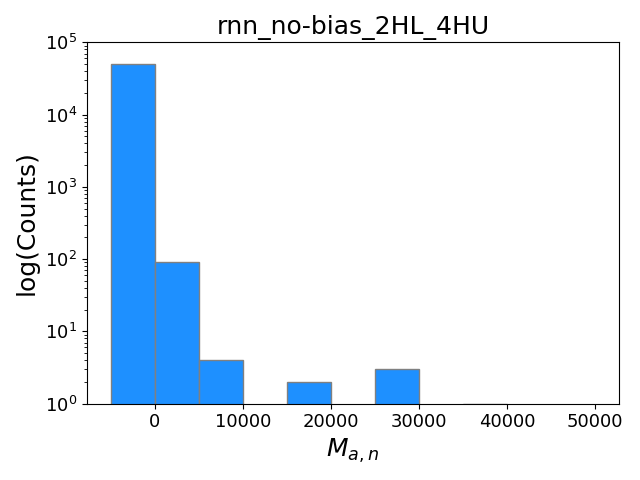
\includegraphics[width=0.3\textwidth]{rnn_no-bias_2HL_4HU/rnn_no-bias_2HL_4HU_all_scores_log_dist_.png}}
  
% RNN bias 0HL
  \subfloat{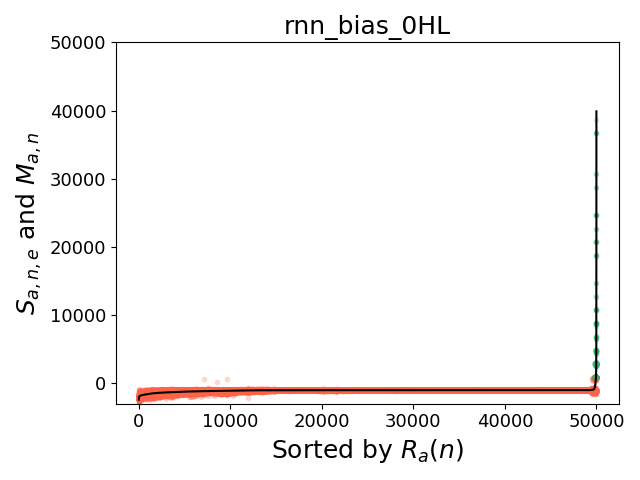
\includegraphics[width=0.3\textwidth]{rnn_bias_0HL/rnn_bias_0HL_score_trials_ordered_.png}}
  \hfill
  \subfloat{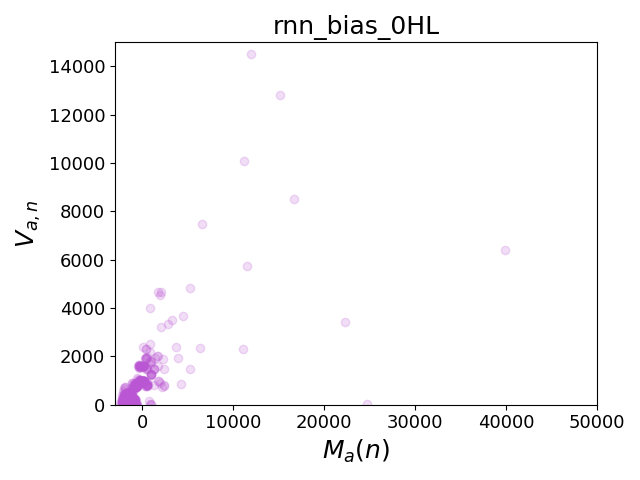
\includegraphics[width=0.3\textwidth]{rnn_bias_0HL/rnn_bias_0HL_variance_meanscore_.png}}
  \hfill
  \subfloat{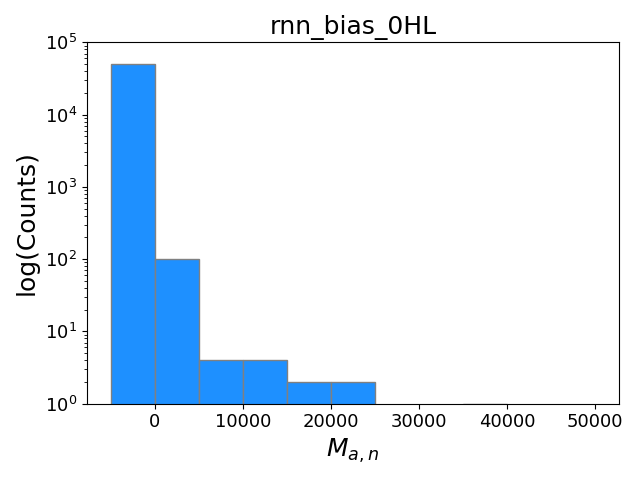
\includegraphics[width=0.3\textwidth]{rnn_bias_0HL/rnn_bias_0HL_all_scores_log_dist_.png}}
  
  % RNN bias 1HL
  \subfloat{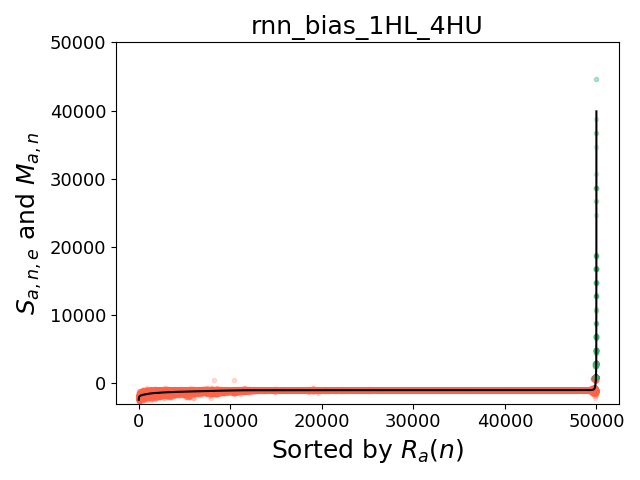
\includegraphics[width=0.3\textwidth]{rnn_bias_1HL_4HU/rnn_bias_1HL_4HU_score_trials_ordered_.png}}
  \hfill
  \subfloat{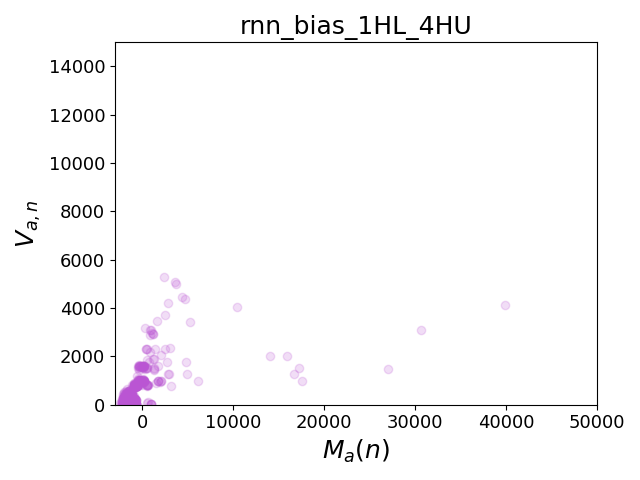
\includegraphics[width=0.3\textwidth]{rnn_bias_1HL_4HU/rnn_bias_1HL_4HU_variance_meanscore_.png}}
  \hfill
  \subfloat{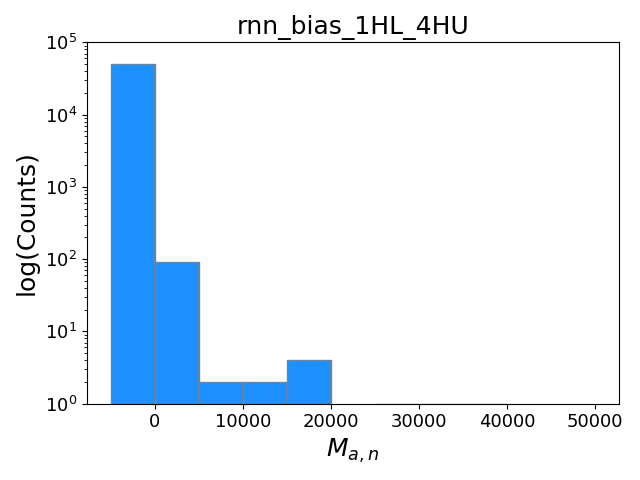
\includegraphics[width=0.3\textwidth]{rnn_bias_1HL_4HU/rnn_bias_1HL_4HU_all_scores_log_dist_.png}}

% RNN bias 2HL
  \subfloat{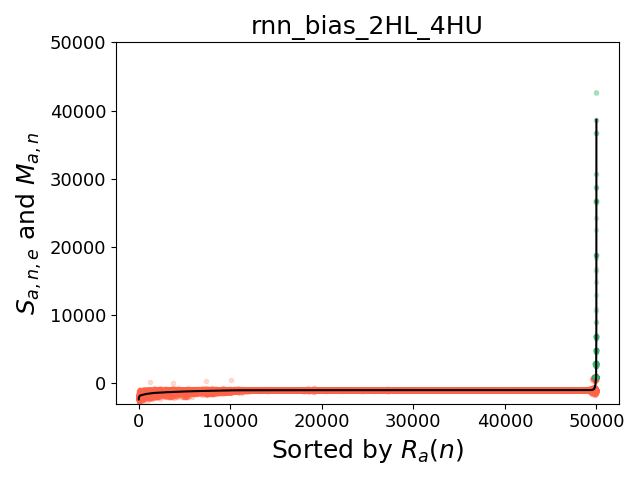
\includegraphics[width=0.3\textwidth]{rnn_bias_2HL_4HU/rnn_bias_2HL_4HU_score_trials_ordered_.png}}
  \hfill
  \subfloat{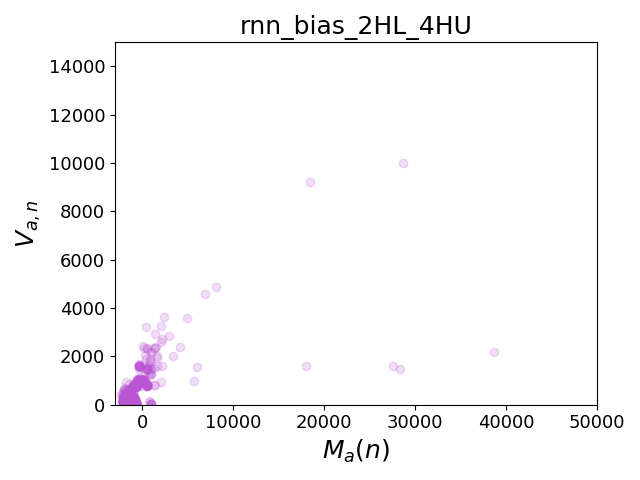
\includegraphics[width=0.3\textwidth]{rnn_bias_2HL_4HU/rnn_bias_2HL_4HU_variance_meanscore_.png}}
  \hfill
  \subfloat{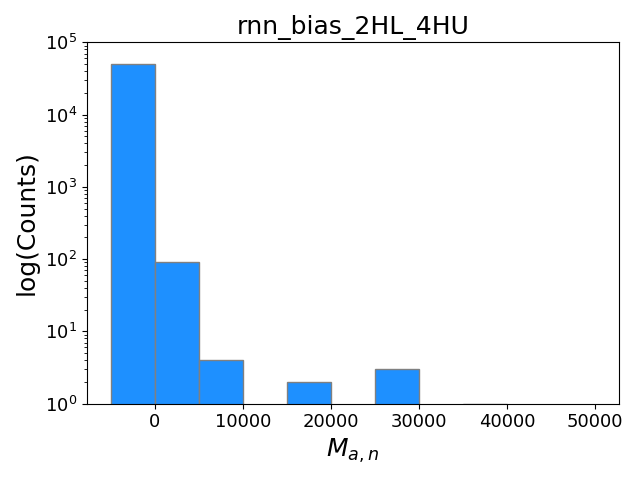
\includegraphics[width=0.3\textwidth]{rnn_bias_2HL_4HU/rnn_bias_2HL_4HU_all_scores_log_dist_.png}}  
  
  \caption{RNN with linear activation}
  \label{fig:rnn_linear}	
\end{figure}	

%%%
	
						
\subsection{Modifying Environmental Factors}

The initial experiments gave us an understanding of why the task is difficult, but they used a specific configuration of the environment. It was important to observe how changing these parameters changed the task difficulty. We varied a) the sliding speed, an approximation of slope angle for a 2D discrete environment, b) the presence of a battery i.e. the cost associated with performing actions, and c) the multi-agent nature.

\subsubsection{Sliding speed}

By default, the environment has sliding speed = 4. This means that when a resource is dropped, it slides 4 tiles per time step. This simulates a slope. The presence of a slope is the environmental factor that makes specialised teams outperform generalist teams. In an environment with no slope, a specialist strategy adds no benefit over a generalist one and may even be worse. Conversely, in an environment with a steeper slope, a specialist strategy could provide an even larger advantage because the slope can get resources to the bottom even faster. We ran experiments with varying sliding speed to observe how it impacts the solutions found. For brevity, we only use one architecture: an RNN with bias, no hidden layers and linear activation.\\

From the plots in Figure \ref{fig:sliding_speed} we find that the sliding speed doesn't make much of a difference to the quality of solutions. It is important to note that while sliding speed is an approximation of slope angle it is not a direct analogue. Slope angle affects the speed at which a resource slides down the slope and the speed at which an agent goes up, but sliding speed only affects the speed of the resource. Since the only successful solutions rwg finds are generalists, the speed at which resources slide doesn't factor into their scores because they never drop resources. Any solutions that do drop resources, don't succeed at the task, so the speed at which those resources slid did not affect their score.\\

We also spotted a minor logical error in the code that causes the cost of moving up/down the slope to be the same regardless of the sliding speed. This does not change the stag hunt dynamic of the environment, however it would more accurately represent a slope if the cost of moving changed with the sliding speed.\\ 

\textbf{Main takeaway: Sliding speed doesn't significantly impact the success of generalist solutions because changing sliding speed doesn't make agents slower or increase the cost of moving up the slope.}

\begin{figure}[!tbp]
  \centering
  % Sliding speed 0
  \subfloat{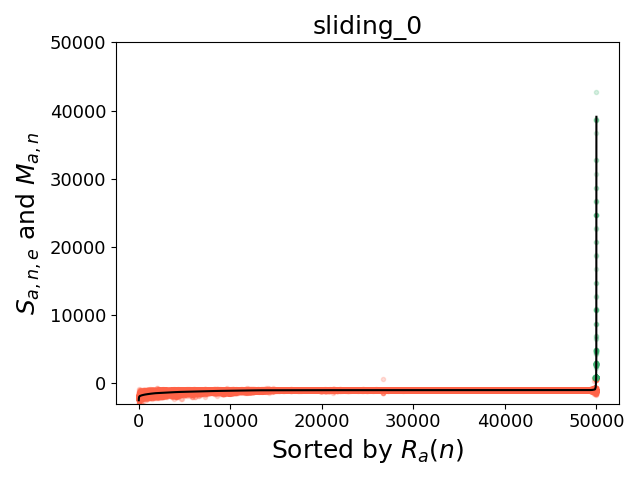
\includegraphics[width=0.3\textwidth]{sliding_0/sliding_0_score_trials_ordered_.png}}
  \hfill
  \subfloat{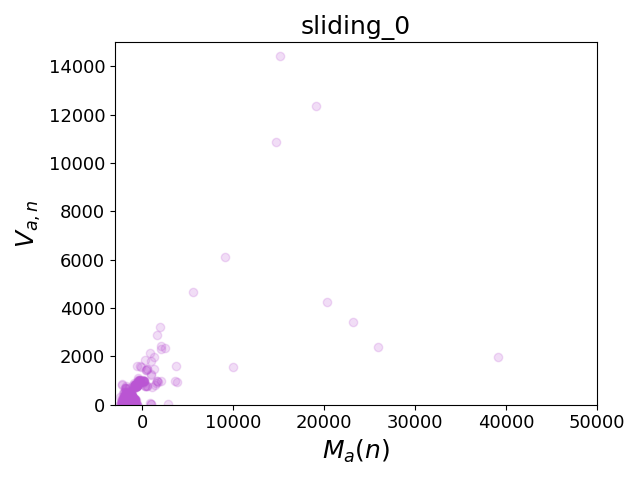
\includegraphics[width=0.3\textwidth]{sliding_0/sliding_0_variance_meanscore_.png}}
  \hfill
  \subfloat{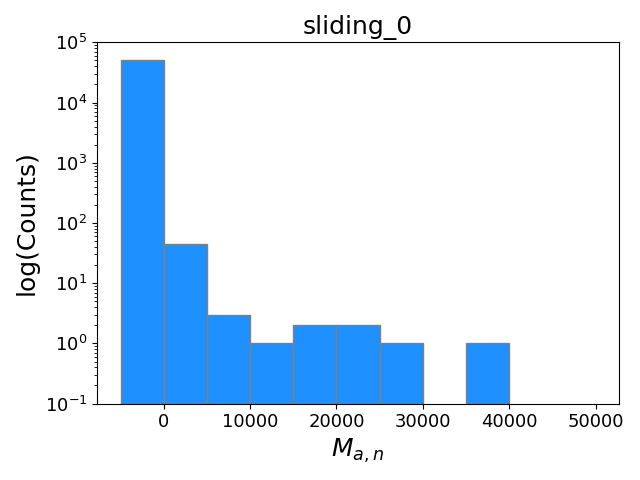
\includegraphics[width=0.3\textwidth]{sliding_0/sliding_0_all_scores_log_dist_.png}}
  
  % Sliding speed 1
  \subfloat{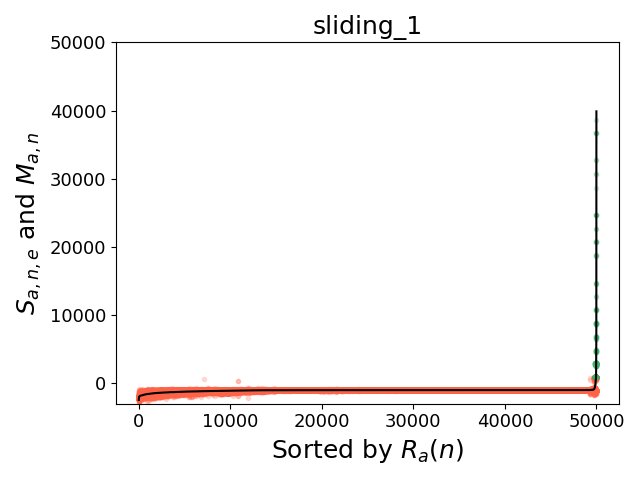
\includegraphics[width=0.3\textwidth]{sliding_1/sliding_1_score_trials_ordered_.png}}
  \hfill
  \subfloat{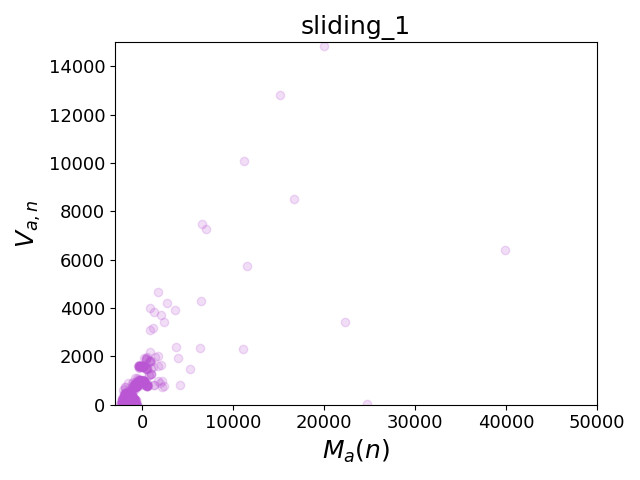
\includegraphics[width=0.3\textwidth]{sliding_1/sliding_1_variance_meanscore_.png}}
  \hfill
  \subfloat{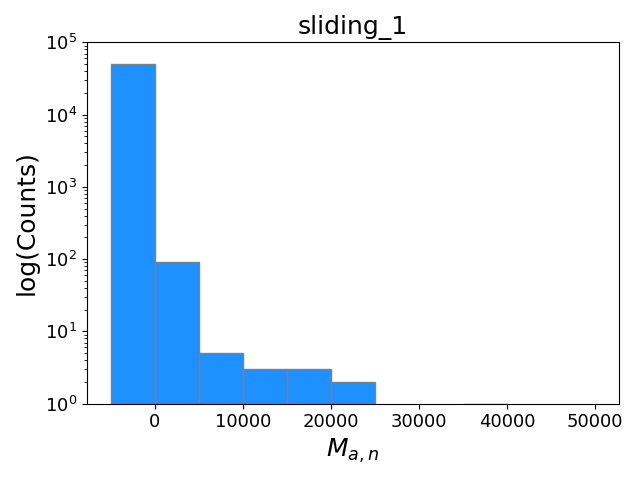
\includegraphics[width=0.3\textwidth]{sliding_1/sliding_1_all_scores_log_dist_.png}}
  
  % Sliding speed 2
  \subfloat{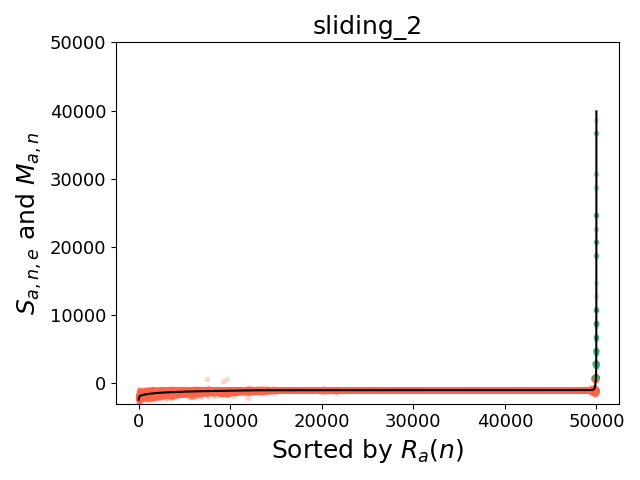
\includegraphics[width=0.3\textwidth]{sliding_2/sliding_2_score_trials_ordered_.png}}
  \hfill
  \subfloat{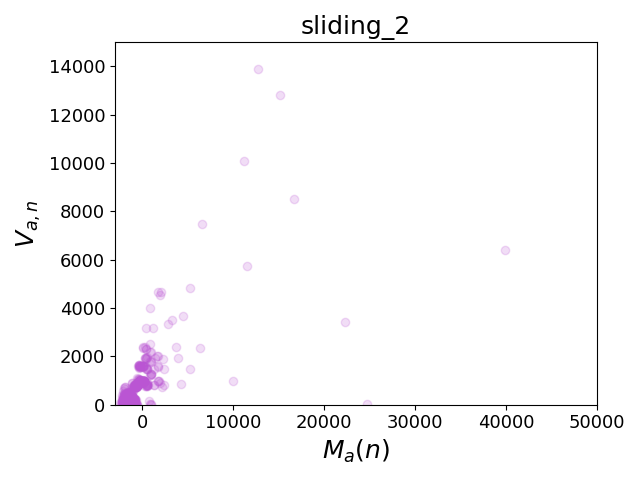
\includegraphics[width=0.3\textwidth]{sliding_2/sliding_2_variance_meanscore_.png}}
  \hfill
  \subfloat{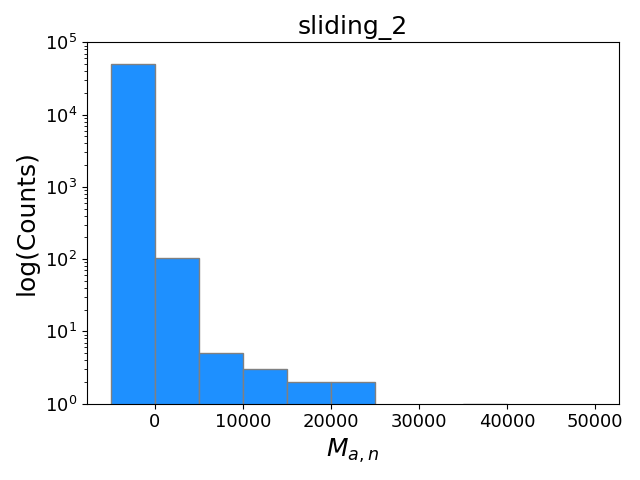
\includegraphics[width=0.3\textwidth]{sliding_2/sliding_2_all_scores_log_dist_.png}}
  
  % Sliding speed 3
  \subfloat{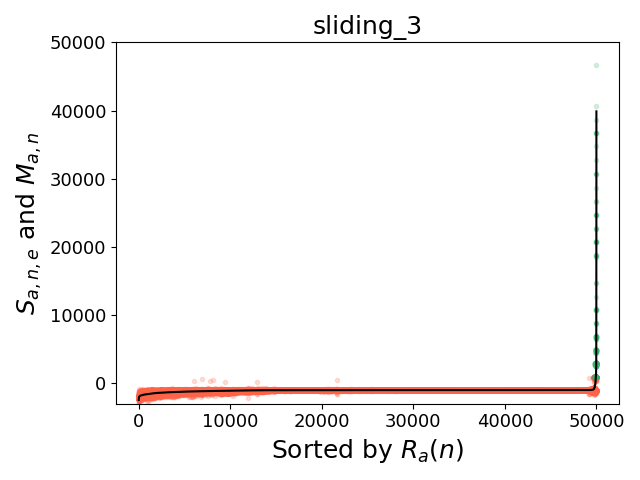
\includegraphics[width=0.3\textwidth]{sliding_3/sliding_3_score_trials_ordered_.png}}
  \hfill
  \subfloat{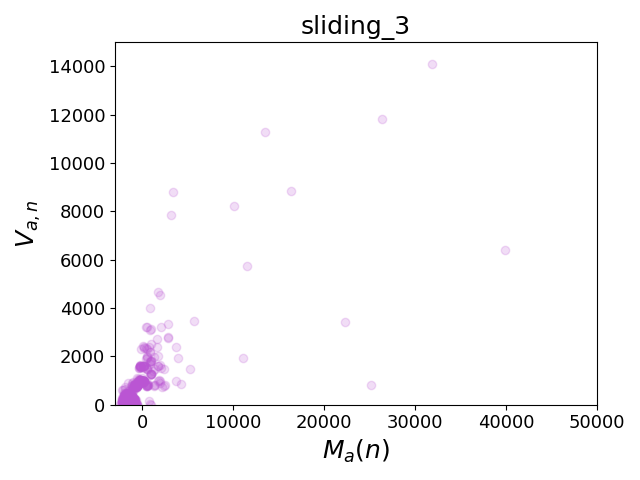
\includegraphics[width=0.3\textwidth]{sliding_3/sliding_3_variance_meanscore_.png}}
  \hfill
  \subfloat{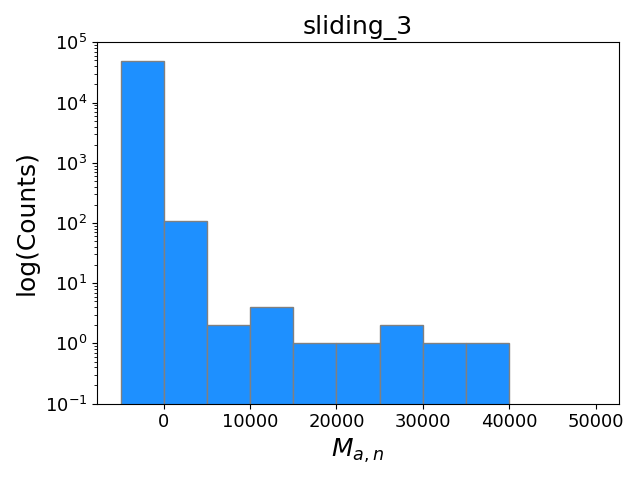
\includegraphics[width=0.3\textwidth]{sliding_3/sliding_3_all_scores_log_dist_.png}}
  
  % Sliding speed 5
  \subfloat{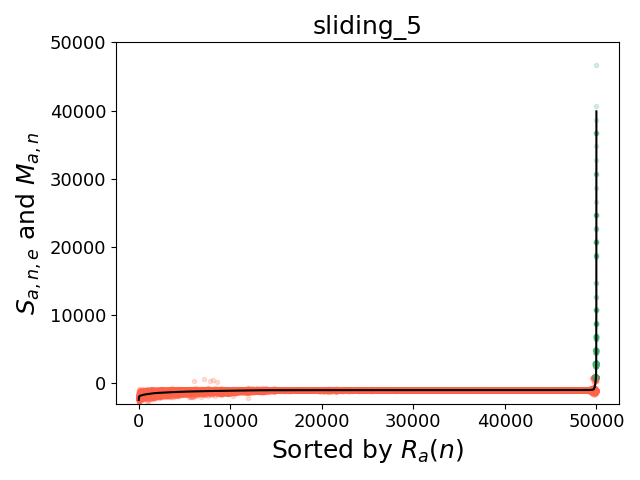
\includegraphics[width=0.3\textwidth]{sliding_5/sliding_5_score_trials_ordered_.png}}
  \hfill
  \subfloat{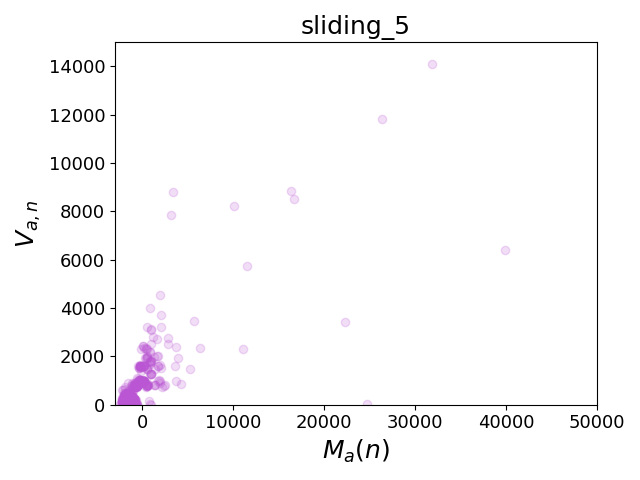
\includegraphics[width=0.3\textwidth]{sliding_5/sliding_5_variance_meanscore_.png}}
  \hfill
  \subfloat{\includegraphics[width=0.3\textwidth]{sliding_5/sliding_5_all_scores_log_dist_.png}}
  
   % Sliding speed 6
  \subfloat{\includegraphics[width=0.3\textwidth]{sliding_6/sliding_6_score_trials_ordered_.png}}
  \hfill
  \subfloat{\includegraphics[width=0.3\textwidth]{sliding_6/sliding_6_variance_meanscore_.png}}
  \hfill
  \subfloat{\includegraphics[width=0.3\textwidth]{sliding_6/sliding_6_all_scores_log_dist_.png}}
  
  \caption{Varying sliding speed}
  \label{fig:sliding_speed}
\end{figure}

\subsubsection{No "battery''}

In our default setup, agents pay a cost for moving in any direction. The cost is higher going up the slope and lower coming down the slope. It is also higher if carrying a resource. This simulates the presence of a battery. An agent is thus, penalised for wasting time and for carrying things on the slope, making specialisation more advantageous and more accurately representing a real robot. A battery is not used by Ferrante et al. \cite{ferrante:2015:PLoSCB} and simply counting the number of resources is sufficient to see specialisation emerge, however, Ferrante et al also had the benefit of 3D physics to create delays in robot and resource movement. It is important to understand how the penalisation of movement impacts the scores of solutions.\\

In the no battery experiments, movement has no cost and agents are rewarded one point for retrieving a resource rather than 1000. We scale down the mean and variance axes in our plots by 1000 to account for this difference. Once again we see in Figure \ref{fig:no_battery} that the majority of solutions are poor, with most retrieving 0 resources. And again we see that variance is higher for the better solutions indicating they are not always successful. There would appear to be more solutions that fall into larger buckets but this is likely only because the scale of the y-axis is smaller, so it is easier for those buckets to be filled. The experiment may need to be repeated with a 1000 score for each retrieved resource.\\

Overall, the absence of a ''battery" or cost to movement does not appear to make any difference to the difficulty of the task which makes sense as the main source of difficulty is the sparseness of the reward. We also know from hardcoded controllers that in the absence of a battery, a specialist team still outperforms a generalist team (scoring 158.4 as opposed to 114.4). The presence or absence of movement and carrying costs does not appear to affect task difficulty.\\

\textbf{Main takeaway: The presence or absence of a ''battery" does not appear to affect task difficulty.}

\begin{figure}[!tbp]
  \centering
  % No battery
  \subfloat{\includegraphics[width=0.3\textwidth]{no_battery/no_battery_score_trials_ordered_.png}}
  \hfill
  \subfloat{\includegraphics[width=0.3\textwidth]{no_battery/no_battery_variance_meanscore_.png}}
  \hfill
  \subfloat{\includegraphics[width=0.3\textwidth]{no_battery/no_battery_all_scores_log_dist_.png}}
  
  \caption{No battery}
  \label{fig:no_battery}
\end{figure}

\subsubsection{Single agent}

\begin{figure}[!tbp]
  \centering
  % Single Agent
  \subfloat{\includegraphics[width=0.3\textwidth]{single_agent/single_agent_score_trials_ordered_.png}}
  \hfill
  \subfloat{\includegraphics[width=0.3\textwidth]{single_agent/single_agent_variance_meanscore_.png}}
  \hfill
  \subfloat{\includegraphics[width=0.3\textwidth]{single_agent/single_agent_all_scores_log_dist_.png}}
  
  \caption{Single agent}
  \label{fig:single_agent}
\end{figure}

\textbf{Main takeaway: }

\subsection{Non-linear Activation}\label{non-linear}

\subsubsection{tanh}

\begin{figure}[!tbp]
  \centering
  % RNN no-bias 0HL
  \subfloat{\includegraphics[width=0.3\textwidth]{rnn_no-bias_0HL_tanh/rnn_no-bias_0HL_tanh_score_trials_ordered_.png}}
  \hfill
  \subfloat{\includegraphics[width=0.3\textwidth]{rnn_no-bias_0HL_tanh/rnn_no-bias_0HL_tanh_variance_meanscore_.png}}
  \hfill
  \subfloat{\includegraphics[width=0.3\textwidth]{rnn_no-bias_0HL_tanh/rnn_no-bias_0HL_tanh_all_scores_log_dist_.png}}
  
  % RNN no-bias 1HL
  \subfloat{\includegraphics[width=0.3\textwidth]{rnn_no-bias_1HL_4HU_tanh/rnn_no-bias_1HL_4HU_tanh_score_trials_ordered_.png}}
  \hfill
  \subfloat{\includegraphics[width=0.3\textwidth]{rnn_no-bias_1HL_4HU_tanh/rnn_no-bias_1HL_4HU_tanh_variance_meanscore_.png}}
  \hfill
  \subfloat{\includegraphics[width=0.3\textwidth]{rnn_no-bias_1HL_4HU_tanh/rnn_no-bias_1HL_4HU_tanh_all_scores_log_dist_.png}}

% RNN no-bias 2HL
  \subfloat{\includegraphics[width=0.3\textwidth]{rnn_no-bias_2HL_4HU_tanh/rnn_no-bias_2HL_4HU_tanh_score_trials_ordered_.png}}
  \hfill
  \subfloat{\includegraphics[width=0.3\textwidth]{rnn_no-bias_2HL_4HU_tanh/rnn_no-bias_2HL_4HU_tanh_variance_meanscore_.png}}
  \hfill
  \subfloat{\includegraphics[width=0.3\textwidth]{rnn_no-bias_2HL_4HU_tanh/rnn_no-bias_2HL_4HU_tanh_all_scores_log_dist_.png}}
  
% RNN bias 0HL
  \subfloat{\includegraphics[width=0.3\textwidth]{rnn_bias_0HL_tanh/rnn_bias_0HL_tanh_score_trials_ordered_.png}}
  \hfill
  \subfloat{\includegraphics[width=0.3\textwidth]{rnn_bias_0HL_tanh/rnn_bias_0HL_tanh_variance_meanscore_.png}}
  \hfill
  \subfloat{\includegraphics[width=0.3\textwidth]{rnn_bias_0HL_tanh/rnn_bias_0HL_tanh_all_scores_log_dist_.png}}
  
  % RNN bias 1HL
  \subfloat{\includegraphics[width=0.3\textwidth]{rnn_bias_1HL_4HU_tanh/rnn_bias_1HL_4HU_tanh_score_trials_ordered_.png}}
  \hfill
  \subfloat{\includegraphics[width=0.3\textwidth]{rnn_bias_1HL_4HU_tanh/rnn_bias_1HL_4HU_tanh_variance_meanscore_.png}}
  \hfill
  \subfloat{\includegraphics[width=0.3\textwidth]{rnn_bias_1HL_4HU_tanh/rnn_bias_1HL_4HU_tanh_all_scores_log_dist_.png}}

% RNN bias 2HL
  \subfloat{\includegraphics[width=0.3\textwidth]{rnn_bias_2HL_4HU_tanh/rnn_bias_2HL_4HU_tanh_score_trials_ordered_.png}}
  \hfill
  \subfloat{\includegraphics[width=0.3\textwidth]{rnn_bias_2HL_4HU_tanh/rnn_bias_2HL_4HU_tanh_variance_meanscore_.png}}
  \hfill
  \subfloat{\includegraphics[width=0.3\textwidth]{rnn_bias_2HL_4HU_tanh/rnn_bias_2HL_4HU_tanh_all_scores_log_dist_.png}}  
  
  \caption{RNN with tanh activation}
  \label{fig:rnn_tanh}	
\end{figure}	

\subsubsection{ReLU}

\begin{figure}[!tbp]
  \centering
  % RNN no-bias 0HL
  \subfloat{\includegraphics[width=0.3\textwidth]{rnn_no-bias_0HL_relu/rnn_no-bias_0HL_relu_score_trials_ordered_.png}}
  \hfill
  \subfloat{\includegraphics[width=0.3\textwidth]{rnn_no-bias_0HL_relu/rnn_no-bias_0HL_relu_variance_meanscore_.png}}
  \hfill
  \subfloat{\includegraphics[width=0.3\textwidth]{rnn_no-bias_0HL_relu/rnn_no-bias_0HL_relu_all_scores_log_dist_.png}}
  
  % RNN no-bias 1HL
  \subfloat{\includegraphics[width=0.3\textwidth]{rnn_no-bias_1HL_4HU_relu/rnn_no-bias_1HL_4HU_relu_score_trials_ordered_.png}}
  \hfill
  \subfloat{\includegraphics[width=0.3\textwidth]{rnn_no-bias_1HL_4HU_relu/rnn_no-bias_1HL_4HU_relu_variance_meanscore_.png}}
  \hfill
  \subfloat{\includegraphics[width=0.3\textwidth]{rnn_no-bias_1HL_4HU_relu/rnn_no-bias_1HL_4HU_relu_all_scores_log_dist_.png}}

% RNN no-bias 2HL
  \subfloat{\includegraphics[width=0.3\textwidth]{rnn_no-bias_2HL_4HU_relu/rnn_no-bias_2HL_4HU_relu_score_trials_ordered_.png}}
  \hfill
  \subfloat{\includegraphics[width=0.3\textwidth]{rnn_no-bias_2HL_4HU_relu/rnn_no-bias_2HL_4HU_relu_variance_meanscore_.png}}
  \hfill
  \subfloat{\includegraphics[width=0.3\textwidth]{rnn_no-bias_2HL_4HU_relu/rnn_no-bias_2HL_4HU_relu_all_scores_log_dist_.png}}
  
% RNN bias 0HL
  \subfloat{\includegraphics[width=0.3\textwidth]{rnn_bias_0HL_relu/rnn_bias_0HL_relu_score_trials_ordered_.png}}
  \hfill
  \subfloat{\includegraphics[width=0.3\textwidth]{rnn_bias_0HL_relu/rnn_bias_0HL_relu_variance_meanscore_.png}}
  \hfill
  \subfloat{\includegraphics[width=0.3\textwidth]{rnn_bias_0HL_relu/rnn_bias_0HL_relu_all_scores_log_dist_.png}}
  
  % RNN bias 1HL
  \subfloat{\includegraphics[width=0.3\textwidth]{rnn_bias_1HL_4HU_relu/rnn_bias_1HL_4HU_relu_score_trials_ordered_.png}}
  \hfill
  \subfloat{\includegraphics[width=0.3\textwidth]{rnn_bias_1HL_4HU_relu/rnn_bias_1HL_4HU_relu_variance_meanscore_.png}}
  \hfill
  \subfloat{\includegraphics[width=0.3\textwidth]{rnn_bias_1HL_4HU_relu/rnn_bias_1HL_4HU_relu_all_scores_log_dist_.png}}

% RNN bias 2HL
  \subfloat{\includegraphics[width=0.3\textwidth]{rnn_bias_2HL_4HU_relu/rnn_bias_2HL_4HU_relu_score_trials_ordered_.png}}
  \hfill
  \subfloat{\includegraphics[width=0.3\textwidth]{rnn_bias_2HL_4HU_relu/rnn_bias_2HL_4HU_relu_variance_meanscore_.png}}
  \hfill
  \subfloat{\includegraphics[width=0.3\textwidth]{rnn_bias_2HL_4HU_relu/rnn_bias_2HL_4HU_relu_all_scores_log_dist_.png}}  
  
  \caption{RNN with relu activation}
  \label{fig:rnn_relu}	
\end{figure}	


\subsubsection{sigmoid}

\begin{figure}[!tbp]
  \centering
  % RNN no-bias 0HL
  \subfloat{\includegraphics[width=0.3\textwidth]{rnn_no-bias_0HL_sigmoid/rnn_no-bias_0HL_sigmoid_score_trials_ordered_.png}}
  \hfill
  \subfloat{\includegraphics[width=0.3\textwidth]{rnn_no-bias_0HL_sigmoid/rnn_no-bias_0HL_sigmoid_variance_meanscore_.png}}
  \hfill
  \subfloat{\includegraphics[width=0.3\textwidth]{rnn_no-bias_0HL_sigmoid/rnn_no-bias_0HL_sigmoid_all_scores_log_dist_.png}}
  
  % RNN no-bias 1HL
  \subfloat{\includegraphics[width=0.3\textwidth]{rnn_no-bias_1HL_4HU_sigmoid/rnn_no-bias_1HL_4HU_sigmoid_score_trials_ordered_.png}}
  \hfill
  \subfloat{\includegraphics[width=0.3\textwidth]{rnn_no-bias_1HL_4HU_sigmoid/rnn_no-bias_1HL_4HU_sigmoid_variance_meanscore_.png}}
  \hfill
  \subfloat{\includegraphics[width=0.3\textwidth]{rnn_no-bias_1HL_4HU_sigmoid/rnn_no-bias_1HL_4HU_sigmoid_all_scores_log_dist_.png}}

% RNN no-bias 2HL
  \subfloat{\includegraphics[width=0.3\textwidth]{rnn_no-bias_2HL_4HU_sigmoid/rnn_no-bias_2HL_4HU_sigmoid_score_trials_ordered_.png}}
  \hfill
  \subfloat{\includegraphics[width=0.3\textwidth]{rnn_no-bias_2HL_4HU_sigmoid/rnn_no-bias_2HL_4HU_sigmoid_variance_meanscore_.png}}
  \hfill
  \subfloat{\includegraphics[width=0.3\textwidth]{rnn_no-bias_2HL_4HU_sigmoid/rnn_no-bias_2HL_4HU_sigmoid_all_scores_log_dist_.png}}
  
% RNN bias 0HL
  \subfloat{\includegraphics[width=0.3\textwidth]{rnn_bias_0HL_sigmoid/rnn_bias_0HL_sigmoid_score_trials_ordered_.png}}
  \hfill
  \subfloat{\includegraphics[width=0.3\textwidth]{rnn_bias_0HL_sigmoid/rnn_bias_0HL_sigmoid_variance_meanscore_.png}}
  \hfill
  \subfloat{\includegraphics[width=0.3\textwidth]{rnn_bias_0HL_sigmoid/rnn_bias_0HL_sigmoid_all_scores_log_dist_.png}}
  
  % RNN bias 1HL
  \subfloat{\includegraphics[width=0.3\textwidth]{rnn_bias_1HL_4HU_sigmoid/rnn_bias_1HL_4HU_sigmoid_score_trials_ordered_.png}}
  \hfill
  \subfloat{\includegraphics[width=0.3\textwidth]{rnn_bias_1HL_4HU_sigmoid/rnn_bias_1HL_4HU_sigmoid_variance_meanscore_.png}}
  \hfill
  \subfloat{\includegraphics[width=0.3\textwidth]{rnn_bias_1HL_4HU_sigmoid/rnn_bias_1HL_4HU_sigmoid_all_scores_log_dist_.png}}

% RNN bias 2HL
  \subfloat{\includegraphics[width=0.3\textwidth]{rnn_bias_2HL_4HU_sigmoid/rnn_bias_2HL_4HU_sigmoid_score_trials_ordered_.png}}
  \hfill
  \subfloat{\includegraphics[width=0.3\textwidth]{rnn_bias_2HL_4HU_sigmoid/rnn_bias_2HL_4HU_sigmoid_variance_meanscore_.png}}
  \hfill
  \subfloat{\includegraphics[width=0.3\textwidth]{rnn_bias_2HL_4HU_sigmoid/rnn_bias_2HL_4HU_sigmoid_all_scores_log_dist_.png}}  
  
  \caption{RNN with sigmoid activation}
  \label{fig:rnn_sigmoid}	
\end{figure}	


\subsubsection{FFNN tanh}

\begin{figure}[!tbp]
  \centering
  % FFNN no-bias 0HL
  \subfloat{\includegraphics[width=0.3\textwidth]{ffnn_no-bias_0HL_tanh/ffnn_no-bias_0HL_tanh_score_trials_ordered_.png}}
  \hfill
  \subfloat{\includegraphics[width=0.3\textwidth]{ffnn_no-bias_0HL_tanh/ffnn_no-bias_0HL_tanh_variance_meanscore_.png}}
  \hfill
  \subfloat{\includegraphics[width=0.3\textwidth]{ffnn_no-bias_0HL_tanh/ffnn_no-bias_0HL_tanh_all_scores_log_dist_.png}}
  
  % FFNN no-bias 1HL
  \subfloat{\includegraphics[width=0.3\textwidth]{ffnn_no-bias_1HL_4HU_tanh/ffnn_no-bias_1HL_4HU_tanh_score_trials_ordered_.png}}
  \hfill
  \subfloat{\includegraphics[width=0.3\textwidth]{ffnn_no-bias_1HL_4HU_tanh/ffnn_no-bias_1HL_4HU_tanh_variance_meanscore_.png}}
  \hfill
  \subfloat{\includegraphics[width=0.3\textwidth]{ffnn_no-bias_1HL_4HU_tanh/ffnn_no-bias_1HL_4HU_tanh_all_scores_log_dist_.png}}

% FFNN no-bias 2HL
  \subfloat{\includegraphics[width=0.3\textwidth]{ffnn_no-bias_2HL_4HU_tanh/ffnn_no-bias_2HL_4HU_tanh_score_trials_ordered_.png}}
  \hfill
  \subfloat{\includegraphics[width=0.3\textwidth]{ffnn_no-bias_2HL_4HU_tanh/ffnn_no-bias_2HL_4HU_tanh_variance_meanscore_.png}}
  \hfill
  \subfloat{\includegraphics[width=0.3\textwidth]{ffnn_no-bias_2HL_4HU_tanh/ffnn_no-bias_2HL_4HU_tanh_all_scores_log_dist_.png}}
  
% FFNN bias 0HL
  \subfloat{\includegraphics[width=0.3\textwidth]{ffnn_bias_0HL_tanh/ffnn_bias_0HL_tanh_score_trials_ordered_.png}}
  \hfill
  \subfloat{\includegraphics[width=0.3\textwidth]{ffnn_bias_0HL_tanh/ffnn_bias_0HL_tanh_variance_meanscore_.png}}
  \hfill
  \subfloat{\includegraphics[width=0.3\textwidth]{ffnn_bias_0HL_tanh/ffnn_bias_0HL_tanh_all_scores_log_dist_.png}}
  
  % FFNN bias 1HL
  \subfloat{\includegraphics[width=0.3\textwidth]{ffnn_bias_1HL_4HU_tanh/ffnn_bias_1HL_4HU_tanh_score_trials_ordered_.png}}
  \hfill
  \subfloat{\includegraphics[width=0.3\textwidth]{ffnn_bias_1HL_4HU_tanh/ffnn_bias_1HL_4HU_tanh_variance_meanscore_.png}}
  \hfill
  \subfloat{\includegraphics[width=0.3\textwidth]{ffnn_bias_1HL_4HU_tanh/ffnn_bias_1HL_4HU_tanh_all_scores_log_dist_.png}}

% FFNN bias 2HL
  \subfloat{\includegraphics[width=0.3\textwidth]{ffnn_bias_2HL_4HU_tanh/ffnn_bias_2HL_4HU_tanh_score_trials_ordered_.png}}
  \hfill
  \subfloat{\includegraphics[width=0.3\textwidth]{ffnn_bias_2HL_4HU_tanh/ffnn_bias_2HL_4HU_tanh_variance_meanscore_.png}}
  \hfill
  \subfloat{\includegraphics[width=0.3\textwidth]{ffnn_bias_2HL_4HU_tanh/ffnn_bias_2HL_4HU_tanh_all_scores_log_dist_.png}}  
  
  \caption{FFNN with tanh activation}
  \label{fig:ffnn_tanh}	
\end{figure}	


\bibliographystyle{plain}
\bibliography{references}

\appendix
\section{The Foraging Task}

We use a foraging task as the testbed for the evolution of specialisation.
The task is modelled off the foraging behaviour of the Atta Leafcutter ant, as in Ferrante et al \cite{ferrante:PLOS_CB:2015} and Pini et al \cite{pini:Swarm_Intelligence:2011; pini:ICSI:2012}.
In nature, the ants cut leaves from a tree and take them to their nest. 
Sometimes the ants partition the task. 
When they do so, some ants are droppers, who cut leaves and let them fall, while other ants are collectors who collect fallen leaves from the base of the tree and take them to the nest.
This partitioned approach is advantageous because gravity transports leaves faster than ants can.
Rather than every ant climbing up the tree, cutting a leaf and bringing it to the nest, when they partition the ants are able to transport more leaves in the same time-span while consuming less energy.
We model this scenario similarly to Ferrante et al \cite{ferrante:PLOS_CB:2015}, with a slope in place of the tree trunk.
Much like the ants, agents transport resources from the source to the nest.
An agent on a team can use a generalist strategy where it acts individually, going up and down the slope to retrieve resources.
An agent can also use a specialist strategy. 
As a specialist it can either be a dropper, going up the slope once and dropping things from the nest, or it can be a collector and gather the resources that accumulate at the base of the slope, called the cache.
Much like real robots that deplete their battery and ants that deplete their energy stores, there is a cost to moving and it is compounded when going up the slope. 
Teams that use complementary specialist strategies pay a smaller energy cost as well as time cost, since resources slide down faster than they can be carried. 
Preliminary analysis with hand-coded agents verifies that specialist teams gain higher overall reward than generalist teams.\\

More formally, you have a team of $n_{agents}$ agents. 
They are placed in a rectangular arena that is $l$ tiles long and $w$ tiles wide, illustrated in Figure \ref{fig:arena}. 
The arena is divided into four sections $l= l_{nest} + l_{cache} + l_{slope} + l_{source}$.
Each episode is composed of a number of finite time-steps $t=0, .... T$. 
Since 3D physics is computationally expensive we use a 2D environment to expedite our experiments as the focus of our research is on the evolutionary process and team dynamics rather than the robotic element.
We also use a discrete scenario, as opposed to a continuous one for further simplicity.
To simulate the presence of gravity, resources move when on the slope, at a speed greater than the agents are capable of.
The high sliding speed creates evolutionary pressure for the team to specialise.
Agents travel at speed $s_{agent}$ and resources slide when placed on the slope with a speed of $s_{resource}$ 
Additionally agents pay costs for moving.
This simulates the presence of a battery, with energy expenditure varying depending on where the agent is moving.
There is a base cost to moving $c$ paid by the agent for moving in any direction.
The base cost is multiplied by different factors for moving up the slope ($f_{up}$) down the slope ($f_{down}$) and moving while carrying a resource ($f_{carry}$). 
An agent moving sideways on the slope pays the same cost as one moving on a non-slope area in any direction.
An agent moving one tile up the slope at time step $t=0$ while carrying a resource, for example, pays a cost of $C_{0} = f_{up} \cdot f_{carry} \cdot c$ .
There are $n_{resources}$ resources at the source, initially.
Every time a resource is removed from the source, another one appears at the source so there are always at least $n_{resources}$.
Each resource retrieved provides all team members a reward of $R$.
The values we chose for these parameters can be found in the appendix\\

Fitness can be calculated for the team or for an individual depending on the level of selection.
When calculating fitness for a team of agents, the fitness function is as follows:\\ 
\\
$F = \sum_{t=1}^{T} \sum_{i}^{n_{agents}} (R_{ti} - C_{ti}) $\\
\\
That is, for each agent, at each time step, we calculate the reward it received at that time step (whether from retrieving a resource itself or from another agent retrieving a resource) and we subtract the cost it individually paid at that time step. 
We then take the summation of this calculation for all agents over all time steps in the simulation.
The reward and cost for an agent $i$ at time step $t$ can be computed as shown here:\\
\\
$
R_{ti} = R \cdot r_{t}
$\\
\\
where $r_t$ is the total number of resources retrieved by all agents at time $t$
\\
\\
\\
$
C_{ti} = \left\{
        \begin{array}{ll}
            c & \quad not on slope or moved sideways on slope\\
            c \cdot f_{up} & \quad up slope\\
            c \cdot f_{down} & \quad down slope\\
            c \cdot f_{carry} & \quad not on slope or moved sideways on slope while carrying\\
            c \cdot f_{carry} \cdot f_{up} & \quad up slope while carrying \\
            c \cdot f_{carry} \cdot f_{down} & \quad down slope while carrying\\
        \end{array}
    \right.
$
\\
\\
When calculating fitness for an individual agent, the fitness function is as follows:\\
\\
$F = \sum_{t=1}^{T} (R_{ti} - C_{ti}) $
\\
\\
Example: Agent 1 incurs -200 retrieving resource. 
Agent 2 incurs -100 wandering around cache. 
Agent 1 score= 1000 - 200. 
Agent 2 score = 1000 - 100.
Team selection: team score = agent 1 score + agent 2 score = 800 + 900 = 1700
Individual selection: agent 1 score = 800, agent 2 score = 900. 
In team selection, team is compared to other teams. 
In individual selection, highest scoring individual is selected. 

\begin{figure}
	\centering
	\includegraphics[width=\textwidth]{arena.jpg}
	\caption{Arena Layout}
	\label{fig:arena}
\end{figure}

\section{Observations and Actions}

Agents have a sensing range that indicates how many tiles around them they can observe. 
A sensing range of 0 means an agent can just observe the current tile it is on. 
A range of 1 means it can observe a square centred  on its location that extends 1 tile in each direction (9 tiles total including current tile). 
A range of 2 means it can observe a square extending 2 tiles in each direction (25 tiles total). 
And so on.
We assume our agent represents a robot with only local sensing capabilities and use a sensing range of 1, which has the added benefit of reducing computation.
For each tile in its sensing range, an agent observes a onehotencoded 4-bit vector. 
The values it reads denote the following: Blank= 1000, Agent = 0100, Resource = 0010, Wall = 0001.
Tiles are read row by row from top left to bottom right. 
The next part of an agent's observation is a 4-bit vector denoting which part of the arena it is on, similar to a real robot with a ground sensor that can detect the unique colour of each area.
The values of this vector can be as follows: Nest = 1000, Cache = 0100, Slope = 0010, Source = 0001
The final part of an agent's observation is 1-bit for resource possession. 
The values can be as follows: Has resource = 1, Doesn’t have resource = 0
The total length of the observation vector is 9x4 + 4 + 1= 41 bits.\\

An agent can perform 6 possible actions, represented by the following values: Forward = 0, Backward = 1, Left = 2, Right = 3, Pick-up = 4, Drop = 5.
We use a recurrent neural network to choose actions based on the observed state.
Since many of the positions in the environment will produce the same observation, a recurrent neural network gives the agent to have a simple form of memory, preventing it from getting "stuck" in infinite state transition loops.
The network has 41 inputs, 1 bias input and 6 recurrent inputs (one for each of the 6 outputs). 
There is no hidden layer, just a 6-neuron output layer. 
This makes for a total of (41+1+6)x6 = 288 weights. 
The output layer uses a linear activation function.

\section{Team Composition and Level of Selection}

During the evolutionary process, it is possible to have four different combinations of team composition and level of selection that impact evolution.
A team can be either homogeneous, with all agents having the same genome, or it can be heterogeneous, with agents having different genomes.
In our case, a heterogeneous team has two different genomes, with half the team having one genome and the other half of the team having the other.
During evolution, team selection can be used, where an entire team of agents can be selected based on the collective fitness of all agents on the team.
Individual selection can also be used, where each agent on the team has its fitness considered separately.
In the latter case, an individual agent with a high reward and low cost can be selected while its team-mates are discarded. 
The four combinations are thus: heterogeneous team with team selection (Het-Team), homogeneous team with team selection (Hom-Team), heterogeneous team with individual selection (Het-Ind) and homogeneous team with individual selection (Hom-Ind).\\


\subsection{Homogeneous Team with Team Selection}

A genome is the weights for one neural network (288 weights) and all agents on a team load that genome into their neural network.
There are 40 teams so 40 genomes are created. 
All members of the team share the reward and cost and a fitness value is returned for the team.
40 fitness values are returned for the whole generation. 
The genome used by the best performing team is selected.\\

\end{document}
